%%%%%%%%%%%%%%%%%%%%%%%%%%%%%%%%%%%%%%%%%
% Beamer Presentation
% LaTeX Template
% Version 1.0 (10/11/12)
%
% This template has been downloaded from:
% http://www.LaTeXTemplates.com
%
% License:
% CC BY-NC-SA 3.0 (http://creativecommons.org/licenses/by-nc-sa/3.0/)
%
%%%%%%%%%%%%%%%%%%%%%%%%%%%%%%%%%%%%%%%%%

%----------------------------------------------------------------------------------------
%	PACKAGES AND THEMES
%----------------------------------------------------------------------------------------

\documentclass{beamer}

\mode<presentation> {

% The Beamer class comes with a number of default slide themes
% which change the colors and layouts of slides. Below this is a list
% of all the themes, uncomment each in turn to see what they look like.

%\usetheme{default}
%\usetheme{AnnArbor}
%\usetheme{Antibes}
%\usetheme{Bergen}
%\usetheme{Berkeley}
%\usetheme{Berlin}
%\usetheme{Boadilla}
%\usetheme{CambridgeUS}
%\usetheme{Copenhagen}
%\usetheme{Darmstadt}
%\usetheme{Dresden}
%\usetheme{Frankfurt}
%\usetheme{Goettingen}
%\usetheme{Hannover}
%\usetheme{Ilmenau}
%\usetheme{JuanLesPins}
%\usetheme{Luebeck}
\usetheme{Madrid}
%\usetheme{Malmoe}
%\usetheme{Marburg}
%\usetheme{Montpellier}
%\usetheme{PaloAlto}
%\usetheme{Pittsburgh}
%\usetheme{Rochester}
%\usetheme{Singapore}
%\usetheme{Szeged}
%\usetheme{Warsaw}

% As well as themes, the Beamer class has a number of color themes
% for any slide theme. Uncomment each of these in turn to see how it
% changes the colors of your current slide theme.

%\usecolortheme{albatross}
%\usecolortheme{beaver}
%\usecolortheme{beetle}
%\usecolortheme{crane}
%\usecolortheme{dolphin}
%\usecolortheme{dove}
%\usecolortheme{fly}
%\usecolortheme{lily}
%\usecolortheme{orchid}
%\usecolortheme{rose}
%\usecolortheme{seagull}
%\usecolortheme{seahorse}
%\usecolortheme{whale}
%\usecolortheme{wolverine}

%\setbeamertemplate{footline} % To remove the footer line in all slides uncomment this line
%\setbeamertemplate{footline}[page number] % To replace the footer line in all slides with a simple slide count uncomment this line

%\setbeamertemplate{navigation symbols}{} % To remove the navigation symbols from the bottom of all slides uncomment this line
}

\usepackage{graphicx} % Allows including images
\usepackage{booktabs} % Allows the use of \toprule, \midrule and \bottomrule in tables
\usepackage{epstopdf}
%----------------------------------------------------------------------------------------
%	TITLE PAGE
%----------------------------------------------------------------------------------------

\title[S.S.C]{Spatial Social Community} % The short title appears at the bottom of every slide, the full title is only on the title page

\author{Lu Chen} % Your name
\institute[FSET] % Your institution as it will appear on the bottom of every slide, may be shorthand to save space
{
Swinburne University of Technology \\ % Your institution for the title page
\medskip
\textit{luchen@swin.edu.au} % Your email address
}
\date{\today} % Date, can be changed to a custom date

\begin{document}

\begin{frame}
\titlepage % Print the title page as the first slide
\end{frame}

\begin{frame}
\frametitle{Overview} % Table of contents slide, comment this block out to remove it
\tableofcontents % Throughout your presentation, if you choose to use \section{} and \subsection{} commands, these will automatically be printed on this slide as an overview of your presentation
\end{frame}

%----------------------------------------------------------------------------------------
%	PRESENTATION SLIDES
%----------------------------------------------------------------------------------------

%------------------------------------------------
\section{Preliminary} % Sections can be created in order to organize your presentation into discrete blocks, all sections and subsections are automatically printed in the table of contents as an overview of the talk
%------------------------------------------------
\subsection{Trusses} % A subsection can be created just before a set of slides with a common theme to further break down your presentation into chunks

\begin{frame}
\frametitle{Trusses}
\begin{definition}
A k-truss is a none-trivial, one-component subgraph such that each edge is reinforced by at least k-2 pairs of edges making a triangle with the edge. (Non-trivial here excludes an isolated vertex as a truss)
\end{definition}
\end{frame}

%------------------------------------------------

\subsection{Triangle connected k-truss}
\begin{frame}
\frametitle{Triangle connected k-truss}
\begin{itemize}
\item k $\ge$ 3 
\item Triangle adjacency: given two triangles, they are adjacent if and they share a common edge
\item Triangle connectivity: given any two triangles $\bigtriangleup_{s}$ and $\bigtriangleup_{t}$ in G, they are connected if there exist a series of triangles $\bigtriangleup_{1},...,\bigtriangleup_{n}$ in G, where n $ge$ 2, such that, $\bigtriangleup_{1} = \bigtriangleup_{s}$, $\bigtriangleup_{n}=\bigtriangleup_{t}$ and for $1\le i< n $, $\bigtriangleup_{i}$ and $\bigtriangleup_{i+1}$ are adjacent 
\end{itemize}
\end{frame}

%------------------------------------------------
\subsection{K-truss community}
\begin{frame}
\frametitle{K-truss community}
\begin{definition}
K-truss community: 1)k-truss, 2)triangle connected, and 3)maximal subgraph
\end{definition}
Basic
\begin{itemize}
\item Edge trussness index: running k-truss decomposition
\item Query k-truss communities from a vertex $v$: running BFS search from edges containing $v$
\end{itemize}
Better
\begin{itemize}
\item TCP index: it is built on top of edge trussness index
\item Query k-truss communities from a vertex $v$: running BFS search from $v$
\end{itemize}
\end{frame}

%------------------------------------------------

\subsection{Finding k-truss communities}
\begin{frame}
\frametitle{Finding k-truss communities}
\begin{itemize}
\item Observation: Given a $k$, a edge $e$ in $G=(V,E)$ can only be contained by at most one k-truss community
\item Finding k-truss communities: For each unvisited edge $e$ with trussness no less than $k$ in $G=(V,E)$, we run BFS from it and during the BFS includes any edge that is unvisited and has trussness no less than $k$.
\item \includegraphics[width=5cm]{trusssample.jpg}
\end{itemize}
\end{frame}

%------------------------------------------------
\section{Spatial Constraints}
%------------------------------------------------

\subsection{An example}
\begin{frame}
	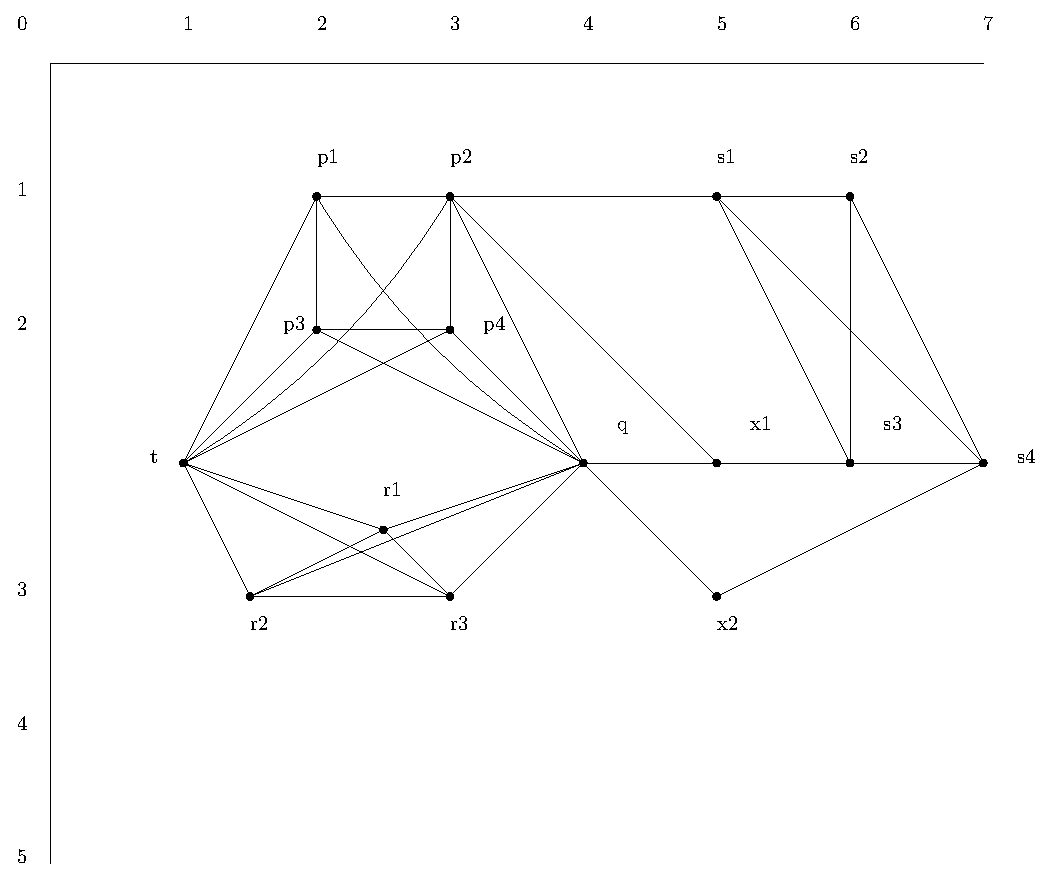
\includegraphics[width=10cm]{sg.eps}
\end{frame}

\subsection{Basic solution}
\begin{frame}
\begin{itemize}
\item Observation: A spatial constrained k-truss community must be contained in a corresponding k-truss community or equal to a corresponding k-truss community 
\item Based on the observation, in the following part, the discussion focuses on finding spatial constrained k-truss communities in a k-truss community.
\item \includegraphics[width=5cm]{trusssample.jpg}
\end{itemize}
\end{frame}

\begin{frame}
\begin{itemize}
\item A k-truss community may contain a set of two-vertexes-pairs. Any pair of vertexes in the set, the distance of the two vertexes is larger than d.
\item Observation: for each pair of vertexes, we only need to remove one of the vertex (different removal choices induce different combinations, which may lead to different results)
\item Observation: For the set of pairs of vertexes, the processing order of pairs of vertexes does not affect the result but affects the performance
\item Observation: After dealing with all pairs of vertexes whose distances are larger than d, the residue of a k-truss community is subgraph of the k-truss community (connected or disconnected).
K-truss communities in the residue are spatial constrained k-truss communities if they exist.
\item 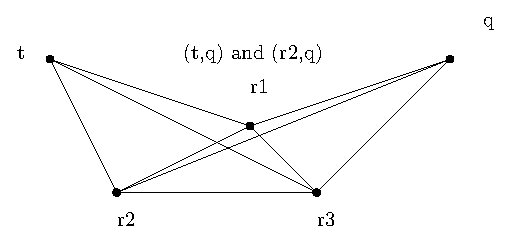
\includegraphics[width=5cm]{subgraph.eps}
\end{itemize}
\end{frame}

\subsection{Algorithm Example}
\begin{frame}
\frametitle{Algorithm Example}
	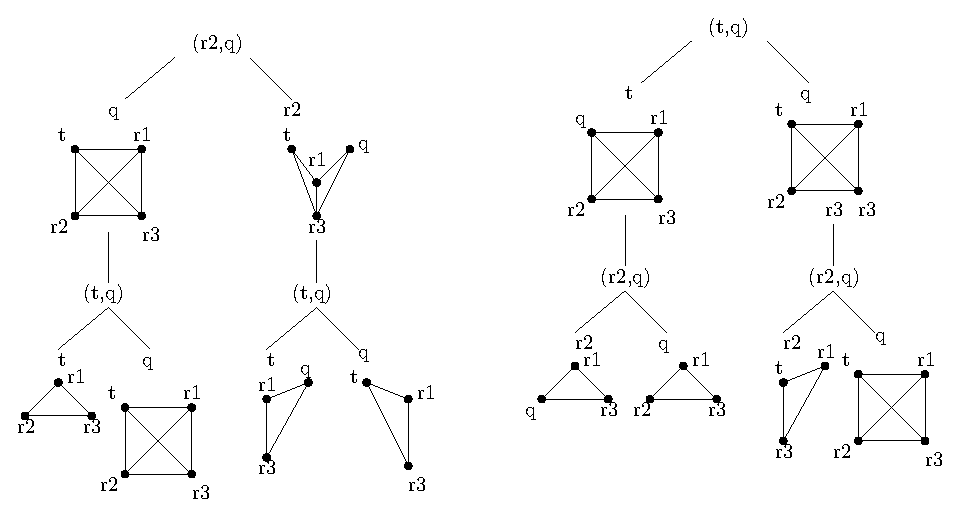
\includegraphics[width=10cm]{re.eps}
\end{frame}

%\begin{frame}
%\frametitle{Table}
%\begin{table}
%\begin{tabular}{l l l}
%\toprule
%\textbf{Treatments} & \textbf{Response 1} & \textbf{Response 2}\\
%\midrule
%Treatment 1 & 0.0003262 & 0.562 \\
%Treatment 2 & 0.0015681 & 0.910 \\
%Treatment 3 & 0.0009271 & 0.296 \\
%\bottomrule
%\end{tabular}
%\caption{Table caption}
%\end{table}
%\end{frame}

%------------------------------------------------


\end{document} 